\documentclass[12pt]{article}
\usepackage[utf8]{inputenc} 
\usepackage{sbc-template}
\usepackage{graphicx,url}
\usepackage{placeins}
\usepackage[brazilian]{babel}


\sloppy

\title{Simulador de monitoramento rebanho bovino \\ utilizando o framework Sinalgo e RMI}

\author{Cristiano Minato\inst{1}, Ricardo Alvim\inst{2} }


\address{Universidade Tecnológica Federal do Paraná
  (UTFPR)\\
  -- Cornélio Procópio -- PR -- Brasil}



\begin{document} 

\maketitle

     
\begin{resumo} 
Nesta trabalho será apresentado um sistema de programação distribuída de sincronização de tarefas em um servidor que fornecerá notificações para o cliente em tempo real, baseado em uma Rede de Sensores Sem Fio, será feito no Sinalgo contendo Nós Sensores (bois) e nós Sink (receptor) para fazer o monitoramento de um rebanho bovino obtendo a identificação de cada boi e sua coordenadas de localização.

\end{resumo}


\section{Introdução}

O Brasil tem uma superfície de aproximadamente 8.515.767,048km² e possui o maior rebanho bovino do mundo, com cerca de 209 milhões de cabeças de gado. Com isso o Brasil assumiu o compromisso da sustentabilidade de carne bovina no mercado. Cerca de 80$\%$ bovino é composta de raças zebuínas que tem uma melhor adaptação ao ambiente no Brasil. A raça que melhor se adaptou foi o Nelore representando uma faixa de 90$\%$ dos bovinos \footnote{Rebanho Brasileiro Bovino. Disponível em: http://www.abiec.com.br/3\underline{ }rebanho.asp. Acessado em 30 out. 2016}.

Para aumentar a produtividade bovina os criadores foram atrás de uma melhor eficiência para a criação de bovinos de corte, uma alternativa foi a criação em confinamento e semi-confinamento. Com isso o desfalque de gados tornou um ponto crítico para os criadores bovinos. Eles tiveram que procurar um mecanismo para inibir esse tipo de ocorrência, um dos mecanismos foi fazer o monitoramento bovino que fosse notificado imediatamente quando houvesse uma ocorrência desse tipo.

As Redes de Sensores Sem Fio são projetadas para sensoriamento remoto de diversos ambientes para medir variáveis do ambiente (temperatura, umidade, luminosidade, posição e etc.) com o objetivo de adquirir dados específicos para cada tipo de situação e em seguida fazer o processamento desses dados para se obter um resultado que possa ser utilizado para tomar alguma decisão.

Neste trabalho vamos apresentar um desenvolvimento de uma rede sem fio para fazer o monitoramento bovino de uma área especifica usando o simulador Sinalgo com nós e sinks, os nós representam o rebanho e os sinks as torres de aquisição e transmissão de dados em uma área previamente definida que por sua vez fornecera a localização de cada animal e se este animal está dentro ou fora da área de pastagem, se o animal estiver fora de sua área de pastagem o proprietário receberá imediatamente uma notificação informando qual o animal está fora de sua área de pastagem.


\section{Conceitos}

    \subsection{Sinalgo}
	Sinalgo é um framework utilizado para fazer simulação e por sua vez é capaz de fazer testes, verificações e validação de algoritmo dentro de uma rede sem fio, más ele não se limita apenas nesta área. Ele oferece uma visão e comunicação da rede. Oferecendo um grande conjunto de condições da rede para você fazer os testes e pode ser usado para aplicações independentes com a finalidade de se obter resultados da simulação \cite{cavalcanteestendendo}.
	
	Para se obter um desempenho satisfatório para a aplicação dos testes e na simplificação na depuração ele foi desenvolvido na linguagem JAVA, oferecendo vários tipos de condições na simulação das redes.
	
	O Sinalgo será usado para gerar os dados referentes ao rebanho bovino, cada bovino será considerado um nó da rede, eles enviarão mensagens contendo seu ID e sua localização no pasto com as coordenadas X e Y. As torres que vão receber as mensagens será considerado como Sinks, eles tem a função de coletar as informações enviadas pelos nó e fazer a verificação de cada nó.
	
	\subsection{Servidores RMI}
	O RMI (Remote Method Invocation) é uma tecnologia suportada pela plataforma Java que facilita o desenvolvimento de aplicações distribuídas. O RMI permite ao programador invocar métodos de objetos remotos, ou seja que estão alojados em máquinas virtuais Java distintas, de uma forma muito semelhante às invocações a objetos locais \footnote{Tutorial RMI - Remote Method Invocation. Disponível em: http://www.devmedia.com.br/tutorial-rmi-remote-method-invocation/6442. Acessado em 30 out. 2016}.. 

	\subsection{Rede de sensores sem fio}
	Redes de Sensores sem Fio (RSSF) são sistemas distribuídos que apresentam vários desafios em muitas áreas de estudo. Uma Rede de Sensores sem Fio (RSSF) é um tipo de rede composta por dispositivos com capacidade de sensoriamento, processamento e comunicação, denominamos nós sensores. Seus dados são recebidos por um ponto de acesso, ou que realizam a ponte de comunicação com outras redes \cite{loureiro2003redes}.
	
    Estas redes têm como objetivo detectar objetos ou fenômenos químicos, físicos ou biológicos em uma determinada área ou região. Possuem dispositivos com capacidade de processamento e energia conectados por uma rede sem fio. Os nós sensores apresentam vantagens como: tamanho reduzido e baixo custo, o que possibilita a distribuição de inúmeros destes sensores em regiões onde o acesso por máquinas ou pessoas é muito difícil ou perigoso \cite{MENEZES:04}.

	

\section{Proposta}
Neste trabalho será desenvolvido um sistema distribuído para fazer o monitoramento de um rebanho bovino. Permitindo que o usuário tenha a identificação e a localização de cada animal do rebanho. Cada animal terá um equipamento para fazer a comunicação e a transmissão de dados para um nó mais próximo dele.

Para fazer essa simulação utilizaremos o Sinalgo e será gerado um nó para cada animal do rebanho, também será gerado sinks que simularão as torres que vão receber os dados, utilizaremos no mínimo 4 sinks para fazer a limitação do pasto, se mesmo assim não conseguimos fazer uma cobertura total do pasto será gerado mais sinks até conseguir uma total cobertura do pasto. Na figura 1 utilizaremos 4 sinks para demonstrar como será feito a limitação do pasto.

\begin{figure}[ht]
	\centering
	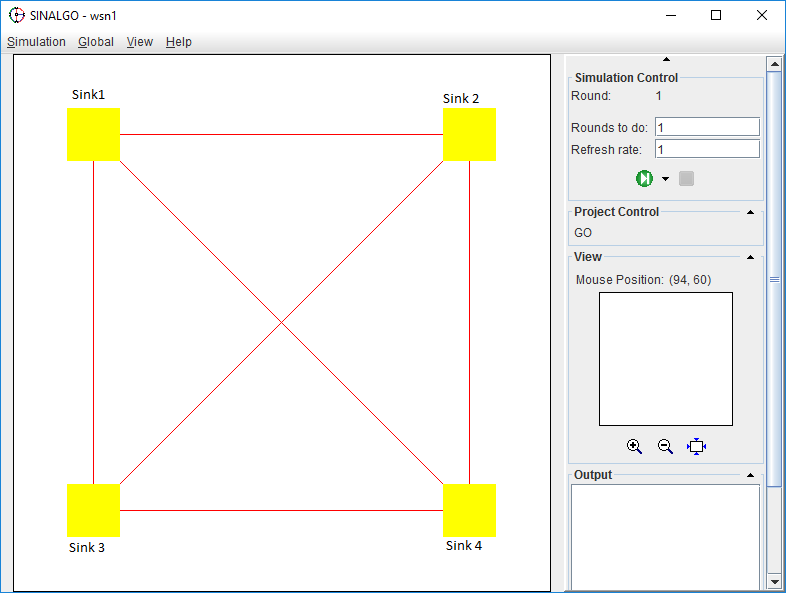
\includegraphics[scale=0.6]{Limite.png}
	\caption{área supervisionada}
	\label{Limite}
\end{figure}
\FloatBarrier 

\subsection{Funcionamento}

O sink vai enviar uma mensagem em broadcast para construir uma rota na qual receberá as mensagens dos nós por essa rota, de tempo em tempo o sink repetirá o procedimento acima para atualizar as rotas para o envio das mensagens. Posteriormente os nós enviarão as mensagens para o sink, nessa mensagem constará o ID e as coordenadas de cada animal do rebanho. Na figura 2 será mostrado os sinks construindo as rotas e na figura 3 a simulação de um nó fora da área de pasto.

\begin{figure}[ht]
	\centering
	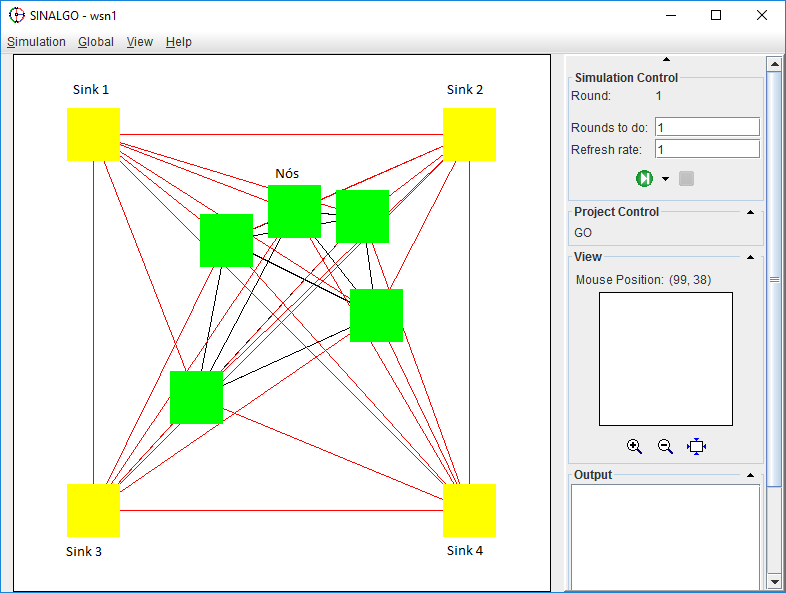
\includegraphics[scale=0.6]{simulacao.png}
	\caption{Simulção utilizando 4 Sinks e 5 nós}
	\label{simulacao}
\end{figure}
\FloatBarrier 

\begin{figure}[ht]
	\centering
	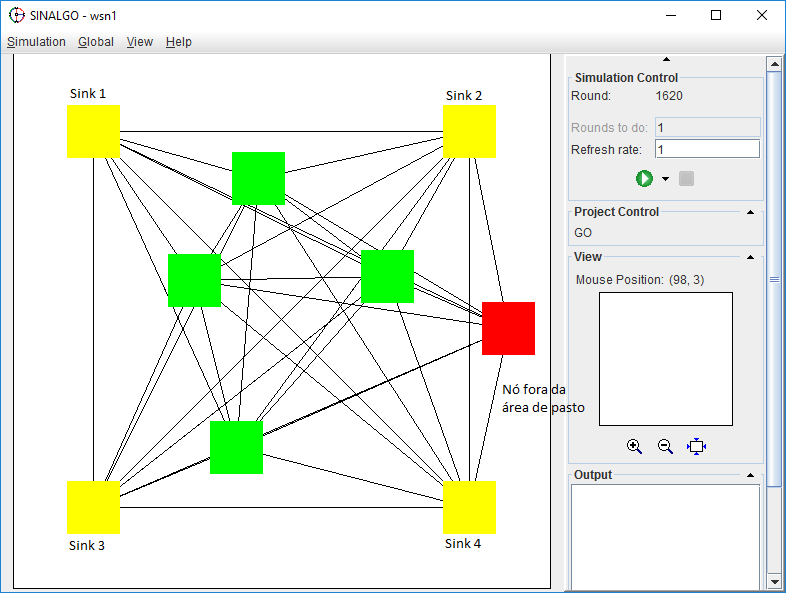
\includegraphics[scale=0.6]{foradopasto.png}
	\caption{Simulção de 1 nós fora da área de pasto}
	\label{foradopasto}
\end{figure}
\FloatBarrier 

\subsection{Classe Cliente}
Essa classe será responsável por obter os dados referente ao rebanho em seguida ele vai mostrar esses dados para o usuário, esses dados são do tipo .txt que é gravado pela classe sink.

\subsection{Classe Servidor}
Essa classe é responsável pela realização da comunicação entre o cliente e os dados e possui uma interface de comunicação em RMI. Ela recebe as mensagens através do sink, e essas mensagens contém as informações dos animais e disponibiliza para o usuário.

\subsection{Classe NodeBovino}
Essa é uma classe que estende de Node, o NodeBovino envia um objeto tipo map, contendo as informações do nó, essa mensagem contém o ID e as coordenadas dele. O método HandleMenssages é responsável por receber e tratar as mensagens recebida, caso seja uma nova mensagem ela é adicionada a uma lista para fazer a verificado mensagem, se tem que enviar a mensagem ou descartar a mensagem se tive que enviar a mensagem para o seu vizinho mais próximo até chegar no sink.

\subsection{Classe NodeSink}
A classe Sink estende os métodos da classe Node, ela envia mensagens em broadcast para criar a rota de comunicação com os nós. Essa classe é responsável por criar as rotas e receber as mensagens enviadas dos nós.

\subsection{Requisitos Funcionais}
Requisitos funcionais são funções que o sistema deve ser capaz de realizar. Abaixo será listado os requisitos funcionais desse software.
- O sistema será capaz de fazer a atualização dos dados na tela sem a intervenção do usuário.
- O sistema deve permitir que o usuário visualize informações de cada animal.
- Deverá fazer o controle de todo o rebanho e informar se algum animal saiu fora da área de pasto previamente demarcada.

\section{Conclusão}
Nesta simulação foram utilizados sensores do tipo nó e sink, a construção das rotas e o envio de mensagens dos nós com suas respectivas informações até o sink está sendo feito a cada 10 rounds, para criação das rotas o sink envia uma mensagem do tipo 0 em broadcast, com essa construção das rotas os nós enviam mensagens para o sink com seu ID e as coordenadas X e Y possibilitando assim o monitoramento bovino. Assim o usuário receberá as informações de seu rebanho bovino em tempo real sobre a situação de seu rebanho, se os animais estão em sua área de pastagem ou se alguns deles estão foram.

\bibliographystyle{sbc}
\bibliography{sbc-template}
\end{document}
